\debut{Emile Martinez}{MPI}{}{}

Dans cette leçon, on illustrera les concepts avec une situation concrètes minimales : un grossiste a une liste de produits dont des clients font la commande.

\begin{personalise}[Objectif]
	Stocker des données de façon à les rendre facilement utilisables, modifiables, etc.
\end{personalise}

\begin{personalise}[Solution naïve]
	Convertir une commande en chaîne de caractères et les stocker dans un grand fichier.
\end{personalise}

\begin{example}
	{ produit : tomate, prix : 3 quantité : 50, client : Le navet naviguant, adresse : 13 rue du Swag à Tarbes },  { produit : patate, prix : 1, quantité : 30, client : Le navet naviguant, adresse : 13 rue du Swag à Tarbes },
\end{example}

\begin{personalise}[Problème]
	Beaucoup de redondances, recherche compliqué
\end{personalise}

\section{Schéma Entité-Association}

\begin{idee}
	Pour éviter les redondances, on stocke à part les clients, les produite. Ensuite on stocke les les liens entre les deux.
\end{idee}

On se place alors dans un paradigme appelé relationnel.

\begin{definition}
	Un schéma entité association est un graphe non orienté composé :
	\begin{itemize}[label=$\star$]
		\item de sommet appelés entités
		\item d'arêtes appelés relations
		\item d'étiquettes sur les arêtes : A une arête $(u,v)$, on associe un étiquette $(x,y)$ ($(v,u)$ sera étiqueté par $(y,x)$) avec $x$ et $y$ pouvant prendre les valeurs : 0..1, 0..*, 1..1 1..*
		\item des attributs sur les sommets et les arêtes précisant ce qu'ils représentent.
	\end{itemize}
\end{definition}

\begin{idee}
	\begin{itemize}
		\item les entités représentent les types des objets (par exemple les clients, les villes, les produits, etc.)
		\item les arêtes représentent les liens (par exemple le fait que un client habite dans telle ville)
		\item les étiquettes sur les arêtes indiquent combien un objet précis peut avoir de liens, la première valeur étant le minimum, la deuxième le maximum ( * représentant donc $+\infty$ )
		\item les attributs représentent les composantes (ex : le nom du client)
	\end{itemize}
\end{idee}

\begin{personalise}[Représentation]
	Les entités sont des carrés, les relations des traits avec un losange au milieu, les étiquettes sont aux bases des arêtes, et les attributs des bulles liés à leur objet.
\end{personalise}

\begin{example}\\
	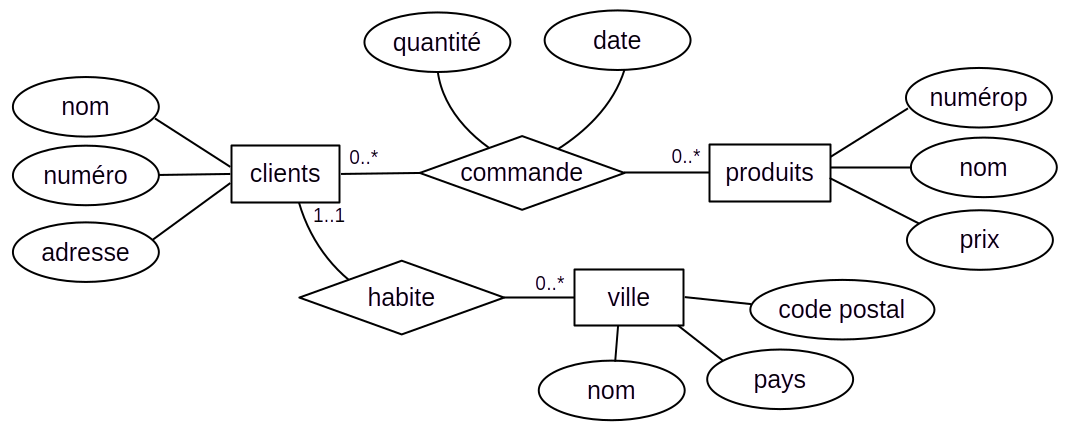
\includegraphics[width=\linewidth]{lecon/27-relationnel-bd/exemple_relationnel.png}
\end{example}

\begin{rem}
	Si on veut que chaque client ait au moins une commande, on met 1..* sur son étiquette associée à commande.
\end{rem}

\begin{proposition}
	On peut convertir les relations ..* ..* en entité
\end{proposition}

\begin{example}\\
	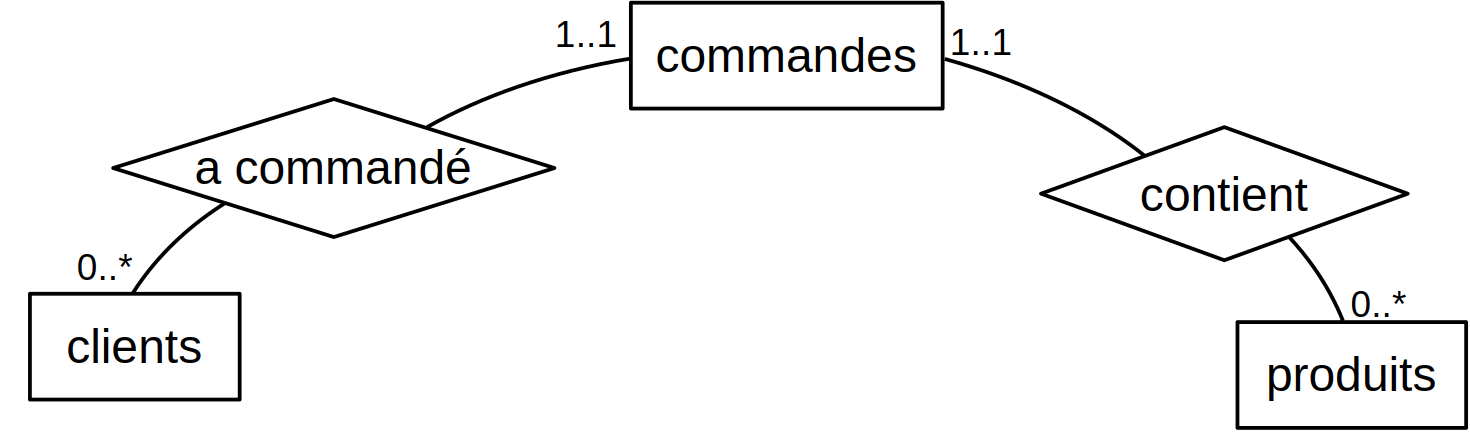
\includegraphics[width=0.8\linewidth]{lecon/27-relationnel-bd/changement_reltionnel.png}
\end{example}

\section{Modèle relationnel}

\subsection{Définitions}

On cherche maintenant une manière de modéliser ce schéma pour le stocker en machine.

\begin{definition}
	\begin{itemize}[label=$\star$]
		\item Un domaine est un ensemble, fini ou non, de valeurs possibles ayant un nom (ex : $(\N, \text{"poids"})$, $(\text{flottant}, \text{"taille"})$, $(\{true, false\}, \text{"present"})$, $(\text{les chaines de caractères}, \text{"nom"})$, etc.)
	
		\item Si $(D1, nom_1), \dots, (D_n, nom_n)$ sont des domaines, on appelle schéma de table (ou schéma de relation) le produit cartésien $D_1 \times D2 \dots \times D_n$ où chaque $D_i$ représente une colonne (ou attributs) représenté par le nom $nom_i$
	
		\item Une table (ou relations) est un sous ensemble du produit cartésien d'un schéma de table.
	
		\item Un enregistrements (ou entrée, ligne, n-uplet) est un élément (donc un n-uplet) d'une table.
	\end{itemize}
\end{definition}

\begin{idee}
	Néanmoins, quand on a un ensemble de tables, on veut qu'elle puisse respecter des règles.
\end{idee}

\begin{example}
	On peut vouloir que les clients mentionnés dans une commande existent en vrai.
\end{example}

\begin{definition}
	\begin{itemize}[label=$\star$]
		\item Une clé d'une table est un ensemble de colonnes tel qu'il n'existe pas deux enregistrements ayant les mêmes valeurs sur ces colonnes.
		
		\item Une clé minimale est une clé qui perd sa propriété si on enlève un attribut
		
		\item Chaque table doit avoir une clé primaire (qui est une clé minimale que l'on choisit)
		
		\item Une clé étrangère est un ensemble de colonne d'une table $t_1$, correspondant à un ensemble de colonnes de $t_2$, et tel que dans tout enregistrement de $t_1$, les $p$-uplets des valeurs des colonnes de la clé étrangère existe dans les colonnes correspondantes de $t_2$.
		
		\item Une contrainte de domaine, imposant à chaque enregistrements d'une table de vérifié une assertion logique.
	\end{itemize}
\end{definition}

\begin{personalise}[Représentation]
	On écrit sous la forme n$om_{table}(attributs1, attributs2, \dots)$ en soulignant les attributs issu d'une clé primaire et en mettant un \# devant les clés étrangères.
\end{personalise}

\begin{example}\\
	\texttt{client(\underline{numero}, nom, \#(code\_postal, pays), adresse)}\\
	\texttt{ville(\underline{code\_postal, pays}, nom)}\\
	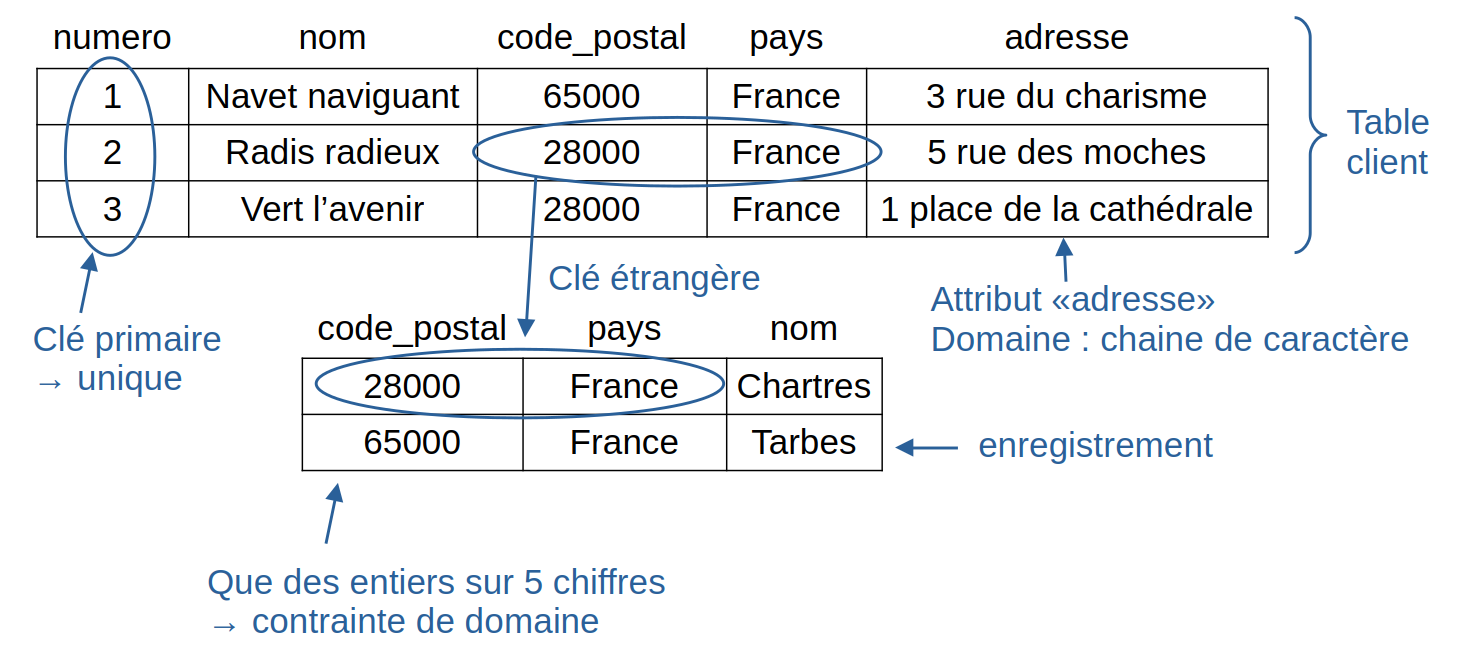
\includegraphics[width=\linewidth]{lecon/27-relationnel-bd/exemple_table.png}
\end{example}

\subsection{De l'entité association au modèle relationnel}

\begin{algo}
	\begin{itemize}[label=$\star$]
		\item Les entités deviennent des relations
		
		\item Pour les associations 1..1 0..* on crée une contrainte de clé étrangère dans la première base vers la clé primaire de la deuxième
		
		\item Pour les associations 0..*  0..* on crée une troisième entité contenant les clés primaires des deux tables, chacune étant des clés étrangères
		
		\item Pour les associations 1..*   1..* on fait la même chose mais les clés étrangères sont dans les tables initiales
		
	\end{itemize}
	
	etc.
\end{algo}

\begin{example}\\
	\texttt{Produit(\underline{numérop}, nom, prix, poids)}\\
	\texttt{Clients(\underline{numéro}, nom, adresse, \#(code\_postal, pays))}\\
	\texttt{Commande(\underline{\#num\_produit, \#num\_client}, quantite)}\\
	\texttt{Ville(\underline{code\_postal, pays}, nom)}
\end{example}

\paragraph{Développement :} Modélisation par une base de données relationnelle d'élèves inscrit à l'université

\section{Implémentation}

\subsection{SGBD}

\begin{definition}
	Un SGBD (système de gestion de bases de données) est un système implémentant les bases de données, permettant d'effectuer des opérations dessus (création, insertion, modification, sélection de certains types de données, etc.) tout en masquant la complexité des opérations.
\end{definition}

\begin{example}
	Exemple de SGBD relationnel : PostgreSQL, MySQL, duckDB, Oracle
\end{example}

\begin{rem}
	Il existe aussi des SGBD ne fonctionnant pas en relationnel. (exemple : IMS)
\end{rem}

\begin{definition}
	 Une transaction est un ensemble d'instruction qui doivent toutes être exécutées ou toutes annulées.
\end{definition}

\begin{example}
	On veut supprimer des produits et donc toutes les commandes attenantes. Si on commence par supprimer par le produit, puis qu'on s'interrompt au milieu de la suppression des commandes,  on aura une base incohérente.
\end{example}

\begin{proposition}
	 Un bon SGBD, doit avoir la propriété ACID pour :
	
	\paragraph{Atomicité :} Une transaction est un tout. Soit tout est fait, soit rien
	
	\paragraph{Cohérence :} Les transactions doivent faire passer la base d'un état cohérent à un autre état cohérent. Les contraintes du modèle relationnel doivent être respectées (clé, clé étrangère, domaine, etc.)
	
	\paragraph{Isolation :} Si deux transactions s'exécutent simultanément, alors leur execution doit produire le même effet que si elle avait était effectué séquentiellement (en particulier, on ne doit pourvoir observer l'état intermédiaire d'une autre transaction)
	
	\paragraph{Durabilité :} Une transaction validé l'est définitivement : un problème (une panne de courant, un cable qui se casse, etc...) ne doit pas mettre à mal la pérennité de la mise à jour.
\end{proposition}

\subsection{SQL}

Pour communiquer avec un SGBD relationnel, a était défini un langage de programmation : le SQL (structured query language).

\begin{rem}
	Ce langage ne dépendant pas de l'implémentation sous-jacente, on ne donne que le résultat que l'on veut et pas la manière de l'obtenir. C'est donc un langage dit déclaratif, dans le paradigme logique.
\end{rem}

\begin{rem}
	Grâce à SQL, les bases de données sont très expressives et donnent de multiples possibilités (théorème de CODD)
\end{rem}

\begin{exercise}
	Trouver le plus de manière possible de chercher le max et faire la division. \label{27-exo-dev2}
\end{exercise}

\paragraph{Développement 2 :} Correction de l'exercice \ref{27-exo-dev2}

\begin{com}
	Ici mettre le développement sur les bases du langages SQL serait plus adaptés à la leçon (en tant qu'introduction à SQL) mais le but étant également de montrer que l'on sait faire des choses, ce développement là est plus intéressant.
\end{com}
